
\documentclass[11pt,a4paper]{article}
\usepackage[utf8]{inputenc}
\usepackage[T1]{fontenc}
\usepackage[spanish,es-nodecimaldot]{babel}
\usepackage[a4paper,left=1.7cm,right=1.7cm,top=20mm,bottom=20mm]{geometry}
\usepackage{amsmath,amssymb,amsfonts,mathtools,bm}
\usepackage{braket}
\usepackage{graphicx}
\usepackage{float}
\usepackage{booktabs}
\usepackage{enumitem}
\usepackage{xcolor}
\usepackage{lmodern,microtype}
\usepackage{fancyhdr}
\usepackage{titlesec}
\usepackage[colorlinks=true,linkcolor=black,urlcolor=black,citecolor=black]{hyperref}
\numberwithin{equation}{section}
\renewcommand{\boxed}[1]{#1}
\setlength{\parindent}{0pt}
\setlength{\parskip}{5pt}
\newcommand{\dd}{\,\mathrm d}
\newcommand{\ii}{\mathrm i}
\newcommand{\e}{\mathrm e}
\newcommand{\hb}{\hbar}
\newcommand{\R}{\mathbb R}
\newcommand{\C}{\mathbb C}
\newcommand{\id}{\mathbb I}

\pagestyle{fancy}
\setlength{\headheight}{14pt}
\fancyhf{}
\fancyhead[L]{\textit{Tarea 5}}
\fancyhead[R]{Física VII: Introducción a la Mecánica Cuántica}
\begin{document}
\begin{titlepage}
\centering
\vspace*{1.8cm}

\includegraphics[width=.22\textwidth]{UdeC_escudo.png}
\vspace{1.1cm}

{\Huge\bfseries Tarea 5\par}
\vspace{.4cm}
{\Huge\bfseries Física VII: Introducción a la Mecánica Cuántica\par}
\vspace{1.5cm}
{\Large José Ignacio Rosas Sepúlveda\par}
\vspace{.8cm}
{\Large Solución\par}
\vfill
\thispagestyle{empty}
\end{titlepage}
\tableofcontents
\newpage
\section*{Enunciado}
\addcontentsline{toc}{section}{Enunciado}
\begin{enumerate}[label=\arabic*.-]
\item Demuestre que las funciones de onda (15) de la clase, asociadas a valores propios distintos $E_n$ y $E_m$, son ortonormales.
\item Demuestre que las funciones de onda (16) de la clase son ortonormales.
\item Encuentre las funciones de onda en representación de momento, $\phi_{n,\pm}(p)$, correspondientes a las funciones propias (16). Grafique la densidad de probabilidad escalada indicada en la clase para $n=1$ y $n=10$.
\item Una partícula de masa $m$ se mueve libremente sobre una trayectoria circular de perímetro $l$. Inicialmente
\begin{equation}
\psi(x,0)=\begin{cases}N,&0\le x\le l/2,\\0,&l/2<x<l,\end{cases}
\end{equation}
donde $N$ es real y positivo.
\begin{enumerate}[label=\alph*)]
\item Encuentre $N$.
\item Encuentre la distribución de probabilidad de proyectar $\psi(x,0)$ sobre las funciones propias (16) y la distribución de energía correspondiente.
\item Encuentre $\psi(x,t)$.
\end{enumerate}
\end{enumerate}
En lo posible, comente sus resultados.


\section{Problemas 1 y 2}
Las funciones de la clase son
\begin{equation}
\phi_{n,\pm}(x)=\frac1{\sqrt l}\e^{\pm\ii2\pi nx/l},\qquad n=0,1,2,\ldots
\end{equation}
Para dos enteros $n,m$ y signos $s,s'\in\{+1,-1\}$,
\begin{equation}
\braket{\phi_{m,s'}|\phi_{n,s}}=
\frac1l\int_0^l\e^{\ii2\pi(sn-s'm)x/l}\dd x.
\end{equation}
La integral vale uno si los exponentes coinciden y cero en caso contrario. Para $n,m>0$ esto prueba la ortonormalidad de los pares degenerados; para $n=0$ las dos notaciones representan el mismo estado constante.

Una base real equivalente para $n\ge1$ es
\begin{equation}
\chi_{n,+}=\sqrt{\frac2l}\cos\frac{2\pi nx}{l},\qquad
\chi_{n,-}=\sqrt{\frac2l}\sin\frac{2\pi nx}{l}.
\end{equation}
Las identidades trigonométricas de producto a suma muestran directamente que
\begin{equation}
\int_0^l\chi_{n,s}(x)\chi_{m,s'}(x)\dd x=\delta_{nm}\delta_{ss'}.
\end{equation}

\section{Problema 3}
Con $q=p/\hb$ y $k_n=2\pi n/l$,
\begin{equation}
\widetilde\chi_{n,+}(p)=\sqrt{\frac{l}{4\pi\hb}}
\left[
\e^{-\ii(q-k_n)l/2}\operatorname{sinc}\frac{(q-k_n)l}{2}
+\e^{-\ii(q+k_n)l/2}\operatorname{sinc}\frac{(q+k_n)l}{2}
\right],
\end{equation}
\begin{equation}
\widetilde\chi_{n,-}(p)=-\ii\sqrt{\frac{l}{4\pi\hb}}
\left[
\e^{-\ii(q-k_n)l/2}\operatorname{sinc}\frac{(q-k_n)l}{2}
-\e^{-\ii(q+k_n)l/2}\operatorname{sinc}\frac{(q+k_n)l}{2}
\right],
\end{equation}
donde $\operatorname{sinc}z=\sin z/z$. La densidad posee máximos alrededor de $p=\pm2\pi n\hb/l$.
\begin{figure}[H]\centering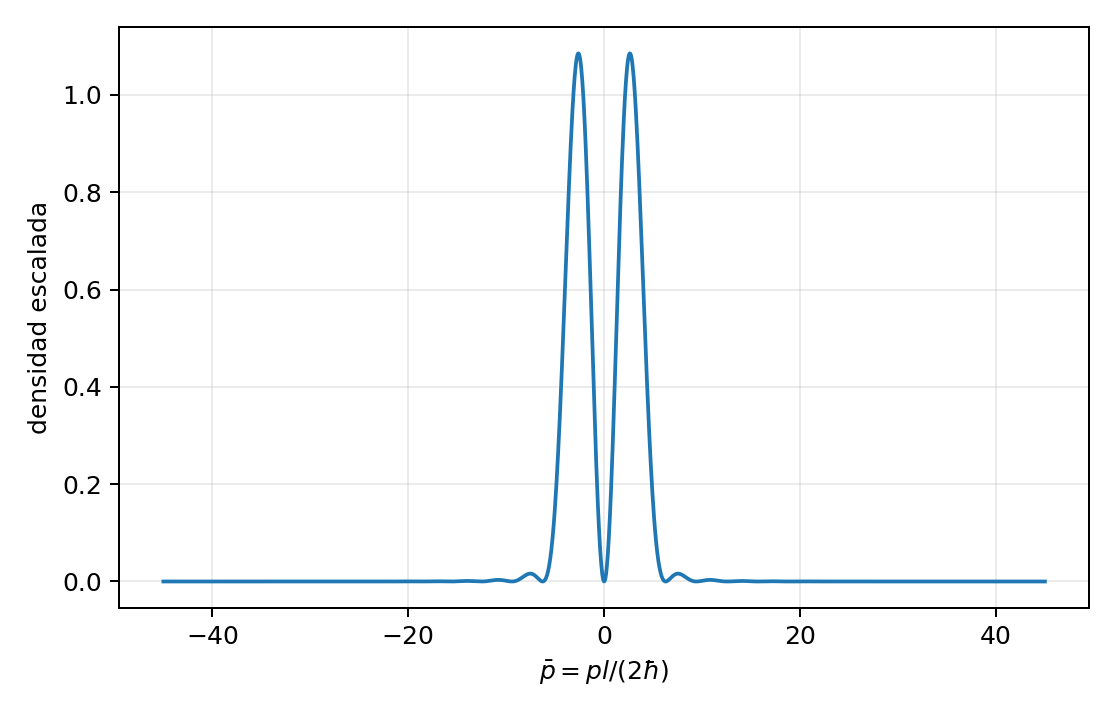
\includegraphics[width=.66\textwidth]{figures/momento_n1.png}\caption{Densidad de momento escalada para $n=1$.}\end{figure}
\begin{figure}[H]\centering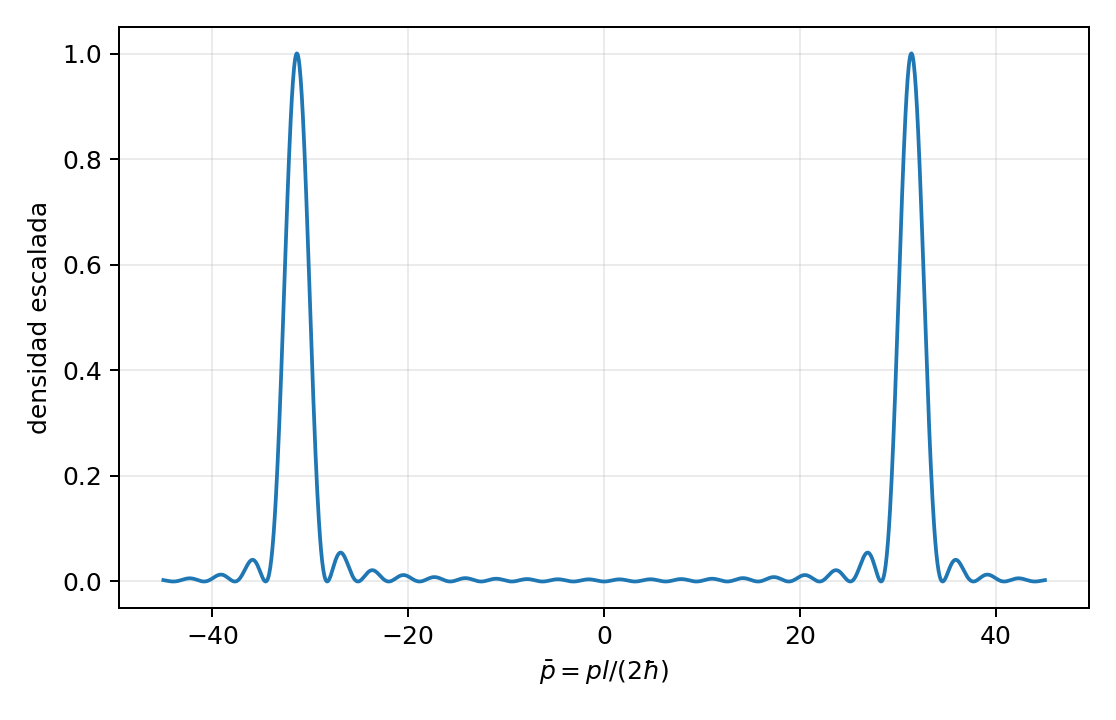
\includegraphics[width=.66\textwidth]{figures/momento_n10.png}\caption{Densidad de momento escalada para $n=10$.}\end{figure}

\section{Problema 4}
La condición inicial es $\psi(x,0)=N$ para $0\le x\le l/2$ y cero en la otra mitad. La normalización entrega
\begin{equation}
\boxed{N=\sqrt{\frac2l}.}
\end{equation}
En la base compleja,
\begin{equation}
c_{n,\pm}=\frac{\sqrt2}{l}\int_0^{l/2}\e^{\mp\ii2\pi nx/l}\dd x.
\end{equation}
Para $n=0$, $c_0=1/\sqrt2$. Para $n\ge1$,
\begin{equation}
c_{n,\pm}=\frac{\sqrt2[(-1)^n-1]}{\mp\ii2\pi n}.
\end{equation}
Por tanto,
\begin{equation}
P(E_0)=\frac12,
\end{equation}
y para $n\ge1$,
\begin{equation}
\boxed{P(E_n)=|c_{n,+}|^2+|c_{n,-}|^2=
\begin{cases}\displaystyle\frac{4}{\pi^2n^2},&n\ \text{impar},\\0,&n\ \text{par}.
\end{cases}}
\end{equation}
La suma es uno porque $\sum_{n\,\mathrm{impar}}1/n^2=\pi^2/8$.

La evolución es
\begin{equation}
\boxed{\psi(x,t)=c_0\phi_0(x)+\sum_{n=1}^{\infty}
\left[c_{n,+}\phi_{n,+}(x)+c_{n,-}\phi_{n,-}(x)\right]\e^{-\ii E_nt/\hb}.}
\end{equation}


\end{document}
